\documentclass{article}
\usepackage[utf8]{inputenc}
\usepackage[english]{babel}
\usepackage[a4paper,top=1.5cm,bottom=1.5cm,left=1.5cm,right=1.5cm,%
bindingoffset=0mm]{geometry}
\usepackage{amssymb}
\usepackage{amsmath}
\newtheorem{prop}{Proposition}
\newtheorem{lemma}{Lemma}
\newenvironment{proof}[1][Proof]{\begin{trivlist}
		\item[\hskip \labelsep {\bfseries #1}]}{\end{trivlist}}
\newcommand{\qed}{\nobreak \ifvmode \relax \else
	\ifdim\lastskip<1.5em \hskip-\lastskip
	\hskip1.5em plus0em minus0.5em \fi \nobreak
	\vrule height0.75em width0.75em depth0em\fi}
\usepackage{tikz}
\usepackage{graphicx}
\def \ourFigPath {../} 
\usepackage{subfigure}
\usepackage{rotating}
\usepackage{float}
\linespread{1.3}
\raggedbottom




%
\font\reali=msbm10 at 12pt
% subsets of real numbers
\newcommand{\real}{\hbox{\reali R}}
\newcommand{\realp}{\hbox{\reali R}_{\scriptscriptstyle +}}
\newcommand{\realpp}{\hbox{\reali R}_{\scriptscriptstyle ++}}
\newcommand{\R}{\mathbb{R}}
\DeclareMathOperator{\E}{\mathbb{E}}
%

\title{General writeup}
\author{Marco Brianti\\Laura Gati}
\date{August 2017}

\begin{document}
	
	\maketitle
	
	\section{VAR Results - Comparison of different specifications}
	
	\subsection{Relative prices LR horizon 8}
	\noindent Time it took, for 500 bootstrap, Mac: 61 min
	
	\noindent  Time it took, for 500 bootstrap, server (w/o parpool): 140 min
	
	\noindent  Time it took, for 500 bootstrap, server (w/ parpool): ? min
	
	\
	
	\noindent  'News'       'IT'        'Total' 
	
         \noindent  '0.17231'    '0.5386'    '0.7109'
         
         
         \
         
         \begin{small}
	\begin{tabular}{lccc}
	\hline
		& News & IT & Total \\
		\hline
		Share of TFP FEV explained & 0.2 & 0.5 & 0.7 \\
		\hline
	\end{tabular}
\end{small}

         
         \

\begin{figure}[h!]
\centering
\subfigure[News]{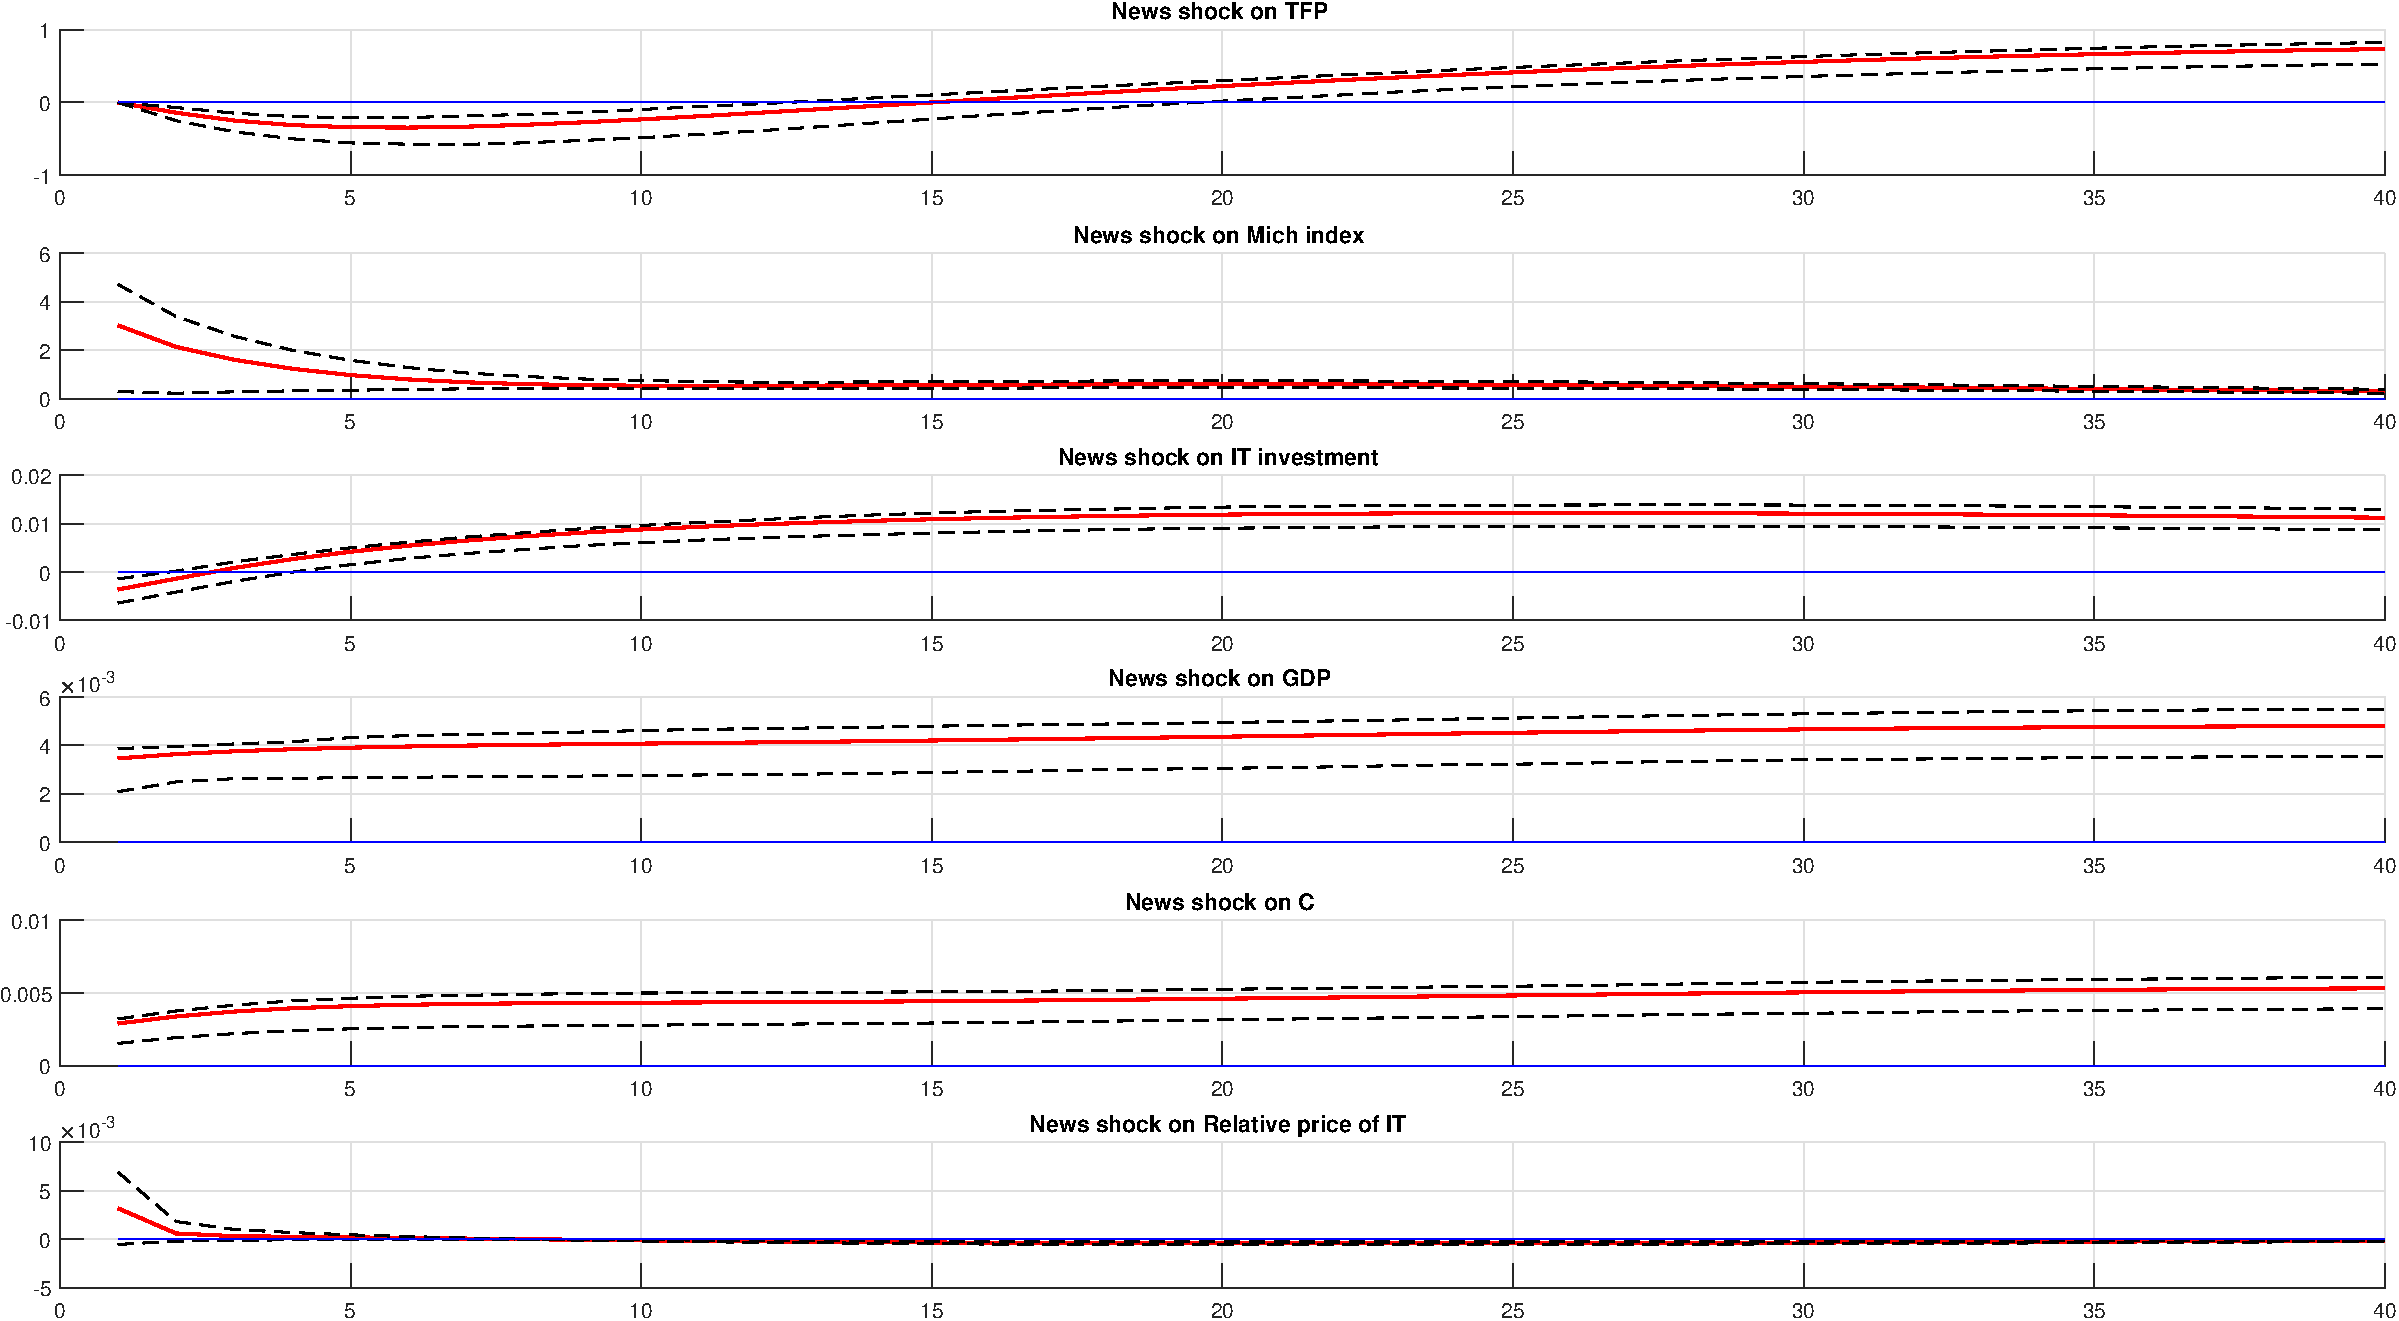
\includegraphics[width=8.5cm]{\ourFigPath Figures/fig_News_shock_Ryan_two_stepsID_20-Nov-2017_12_24_34}} \hspace{.2in%
} 
\subfigure[IT]{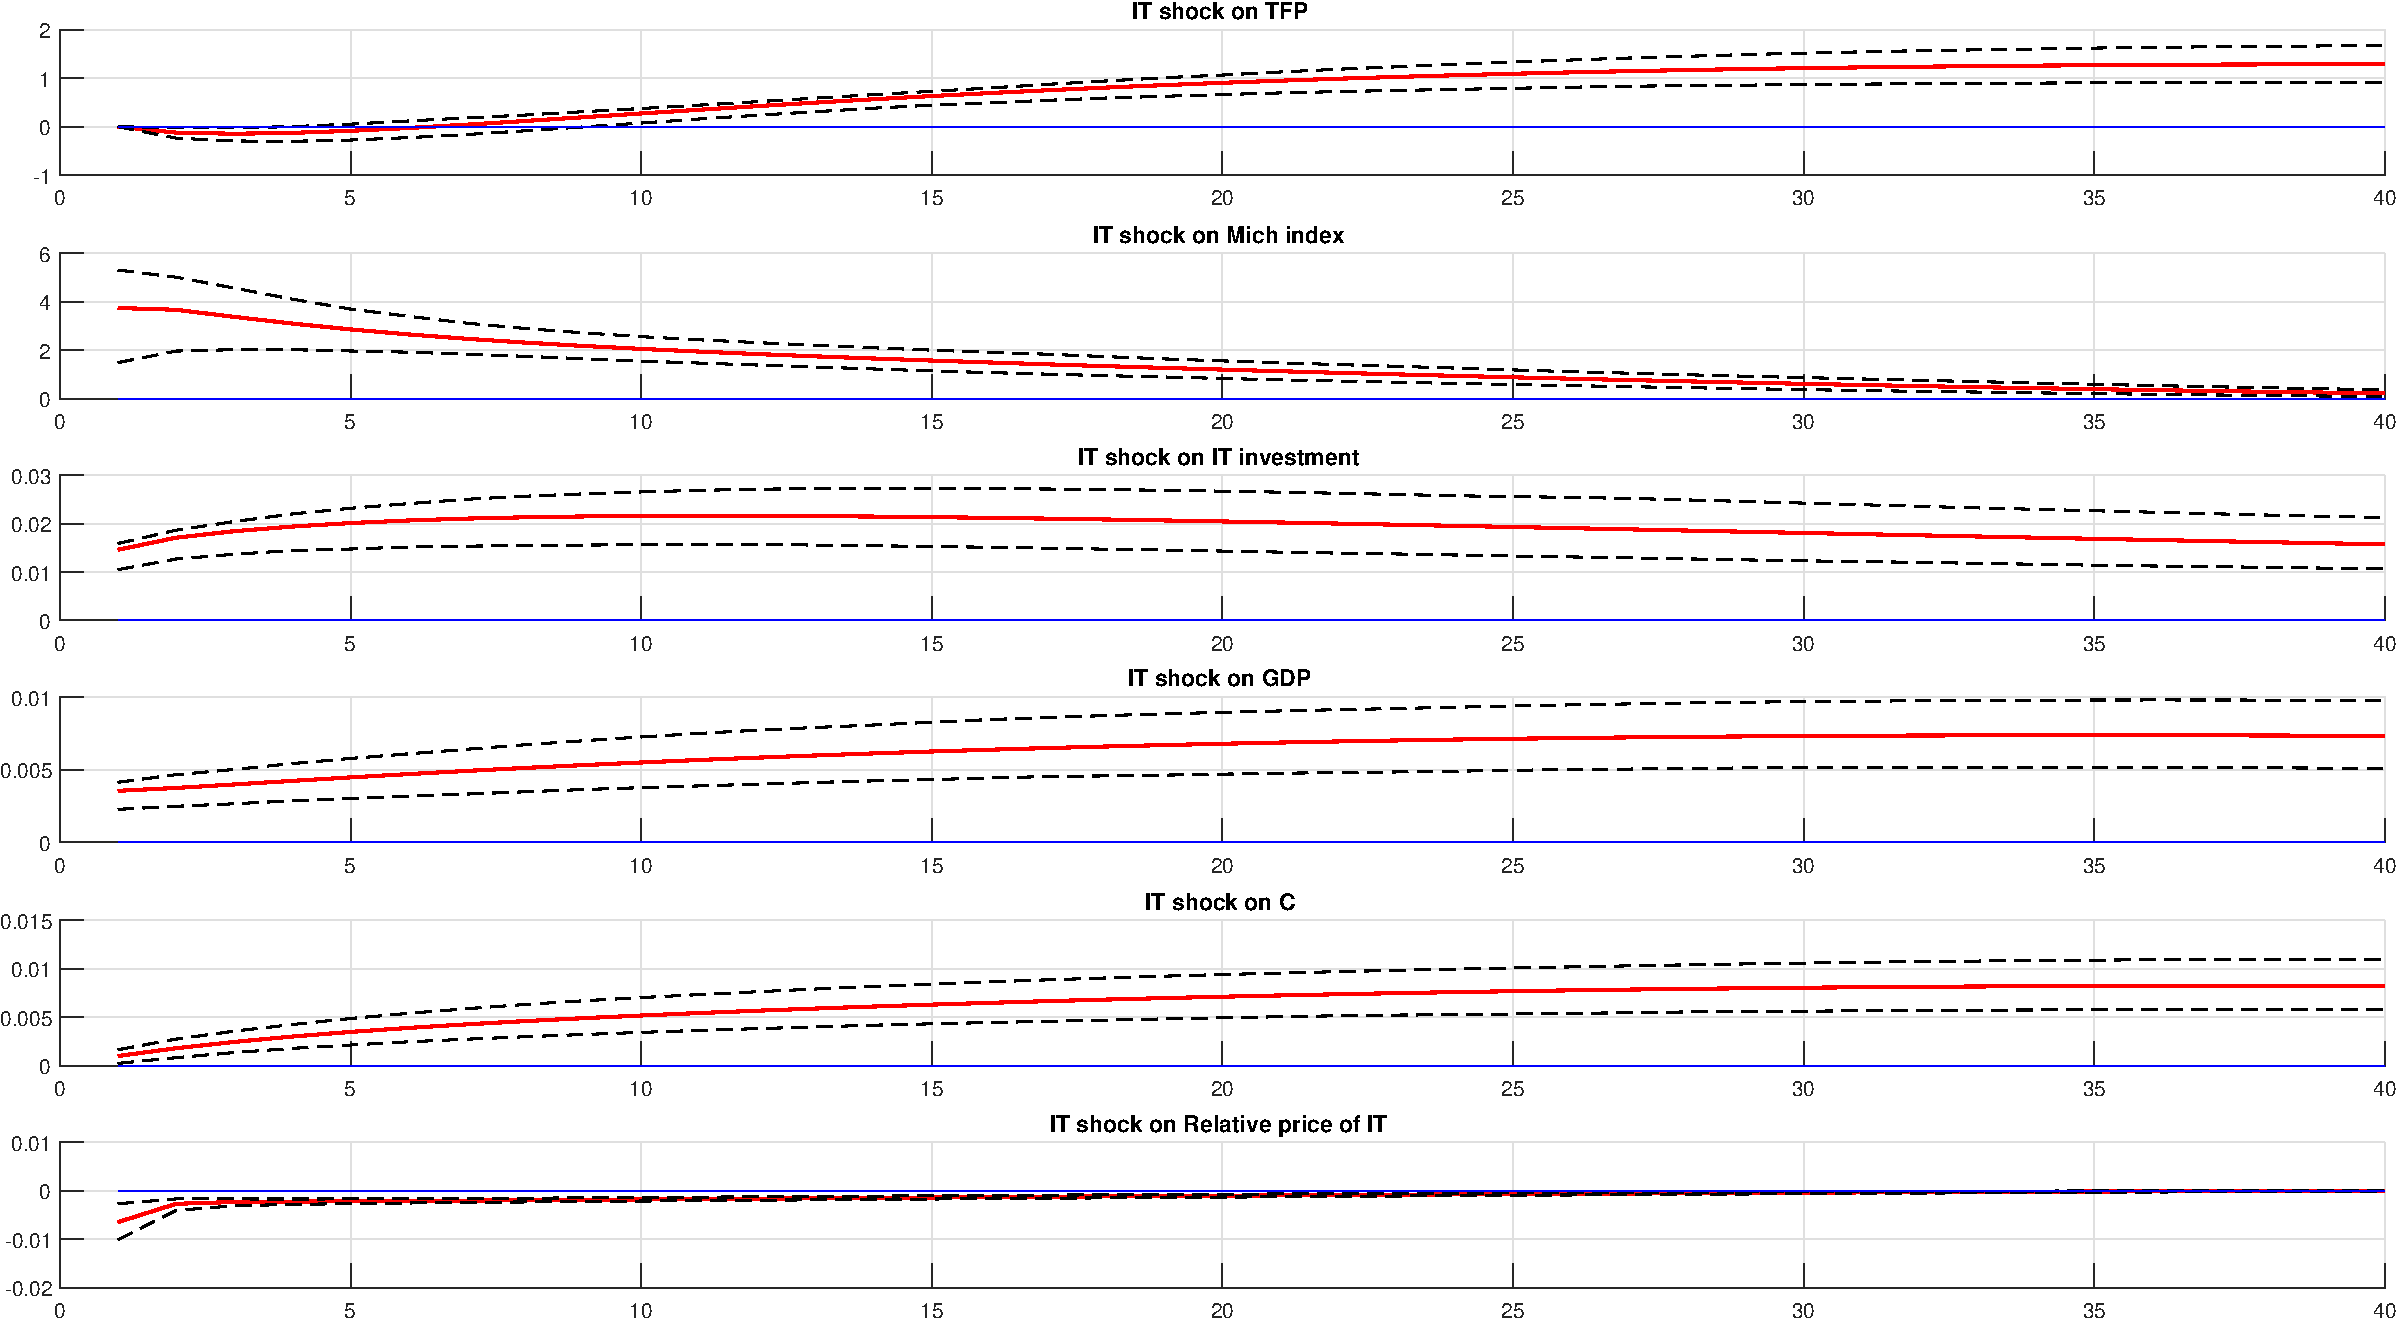
\includegraphics[width=8.5cm]{\ourFigPath Figures/fig_IT_shock_Ryan_two_stepsID_20-Nov-2017_12_24_39}}
\end{figure}
 
%%%%%%%%
% LR hor of 16 
\newpage
\subsection{Relative prices LR horizon 16}
	\noindent Time it took, for 500 bootstrap, Mac: 61 min
	
	\
	
	\noindent  'News'       'IT'        'Total' 
	
         \noindent  '0.10054'    '0.60847'    '0.70901'
         
         \
         
         \begin{small}
	\begin{tabular}{lccc}
	\hline
		& News & IT & Total \\
		\hline
		Share of TFP FEV explained & 0.1 & 0.6 & 0.7 \\
		\hline
	\end{tabular}
\end{small}

         
         \

\begin{figure}[h!]
\centering
\subfigure[News]{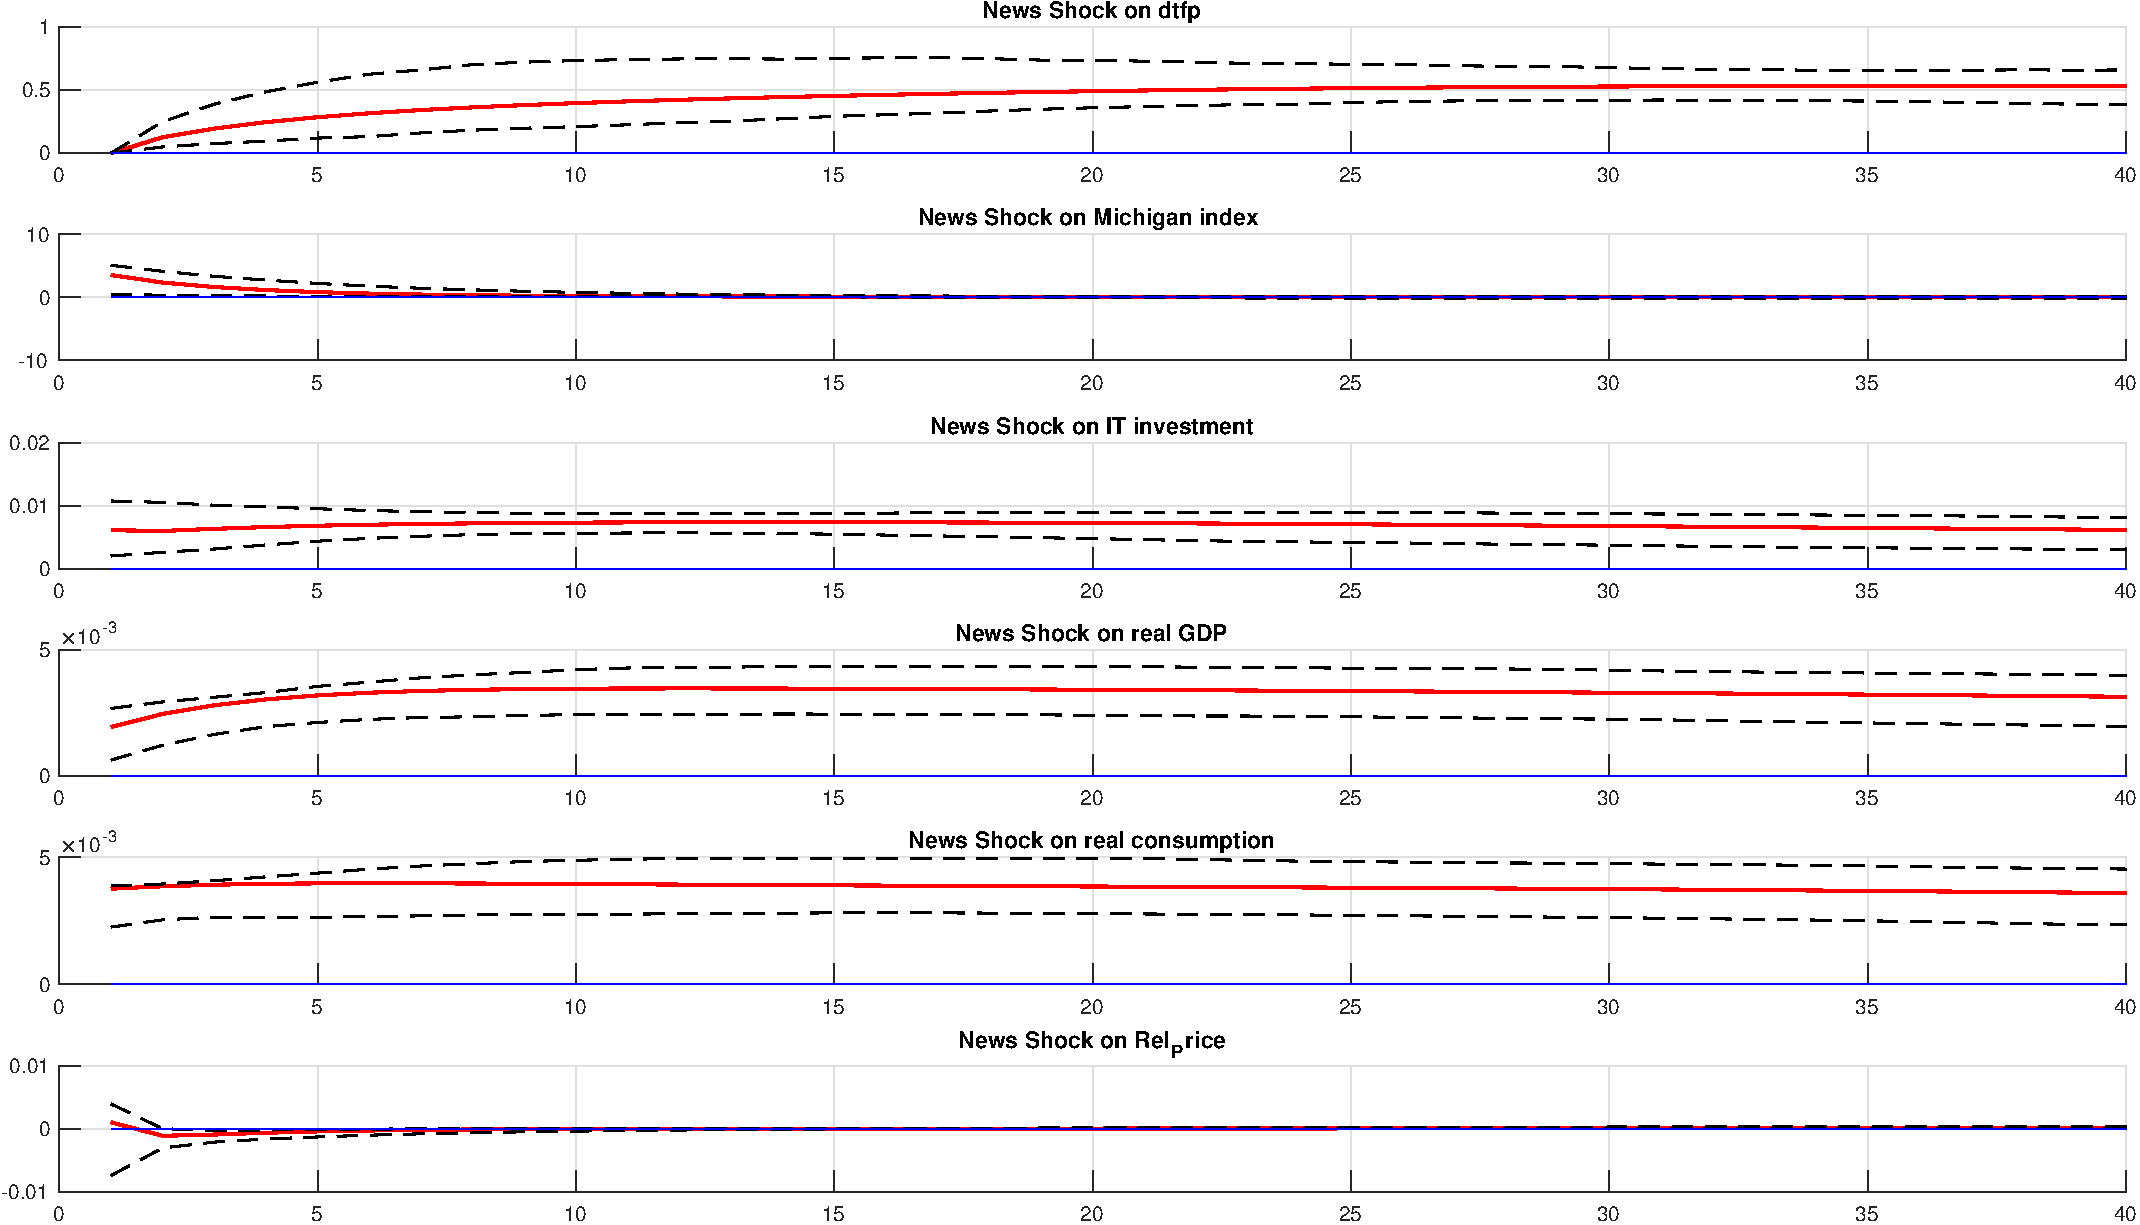
\includegraphics[width=8.5cm]{\ourFigPath Figures/fig_News_Shock_Ryan_two_stepsID_24-Nov-2017_18_56_19}} \hspace{.2in%
} 
\subfigure[IT]{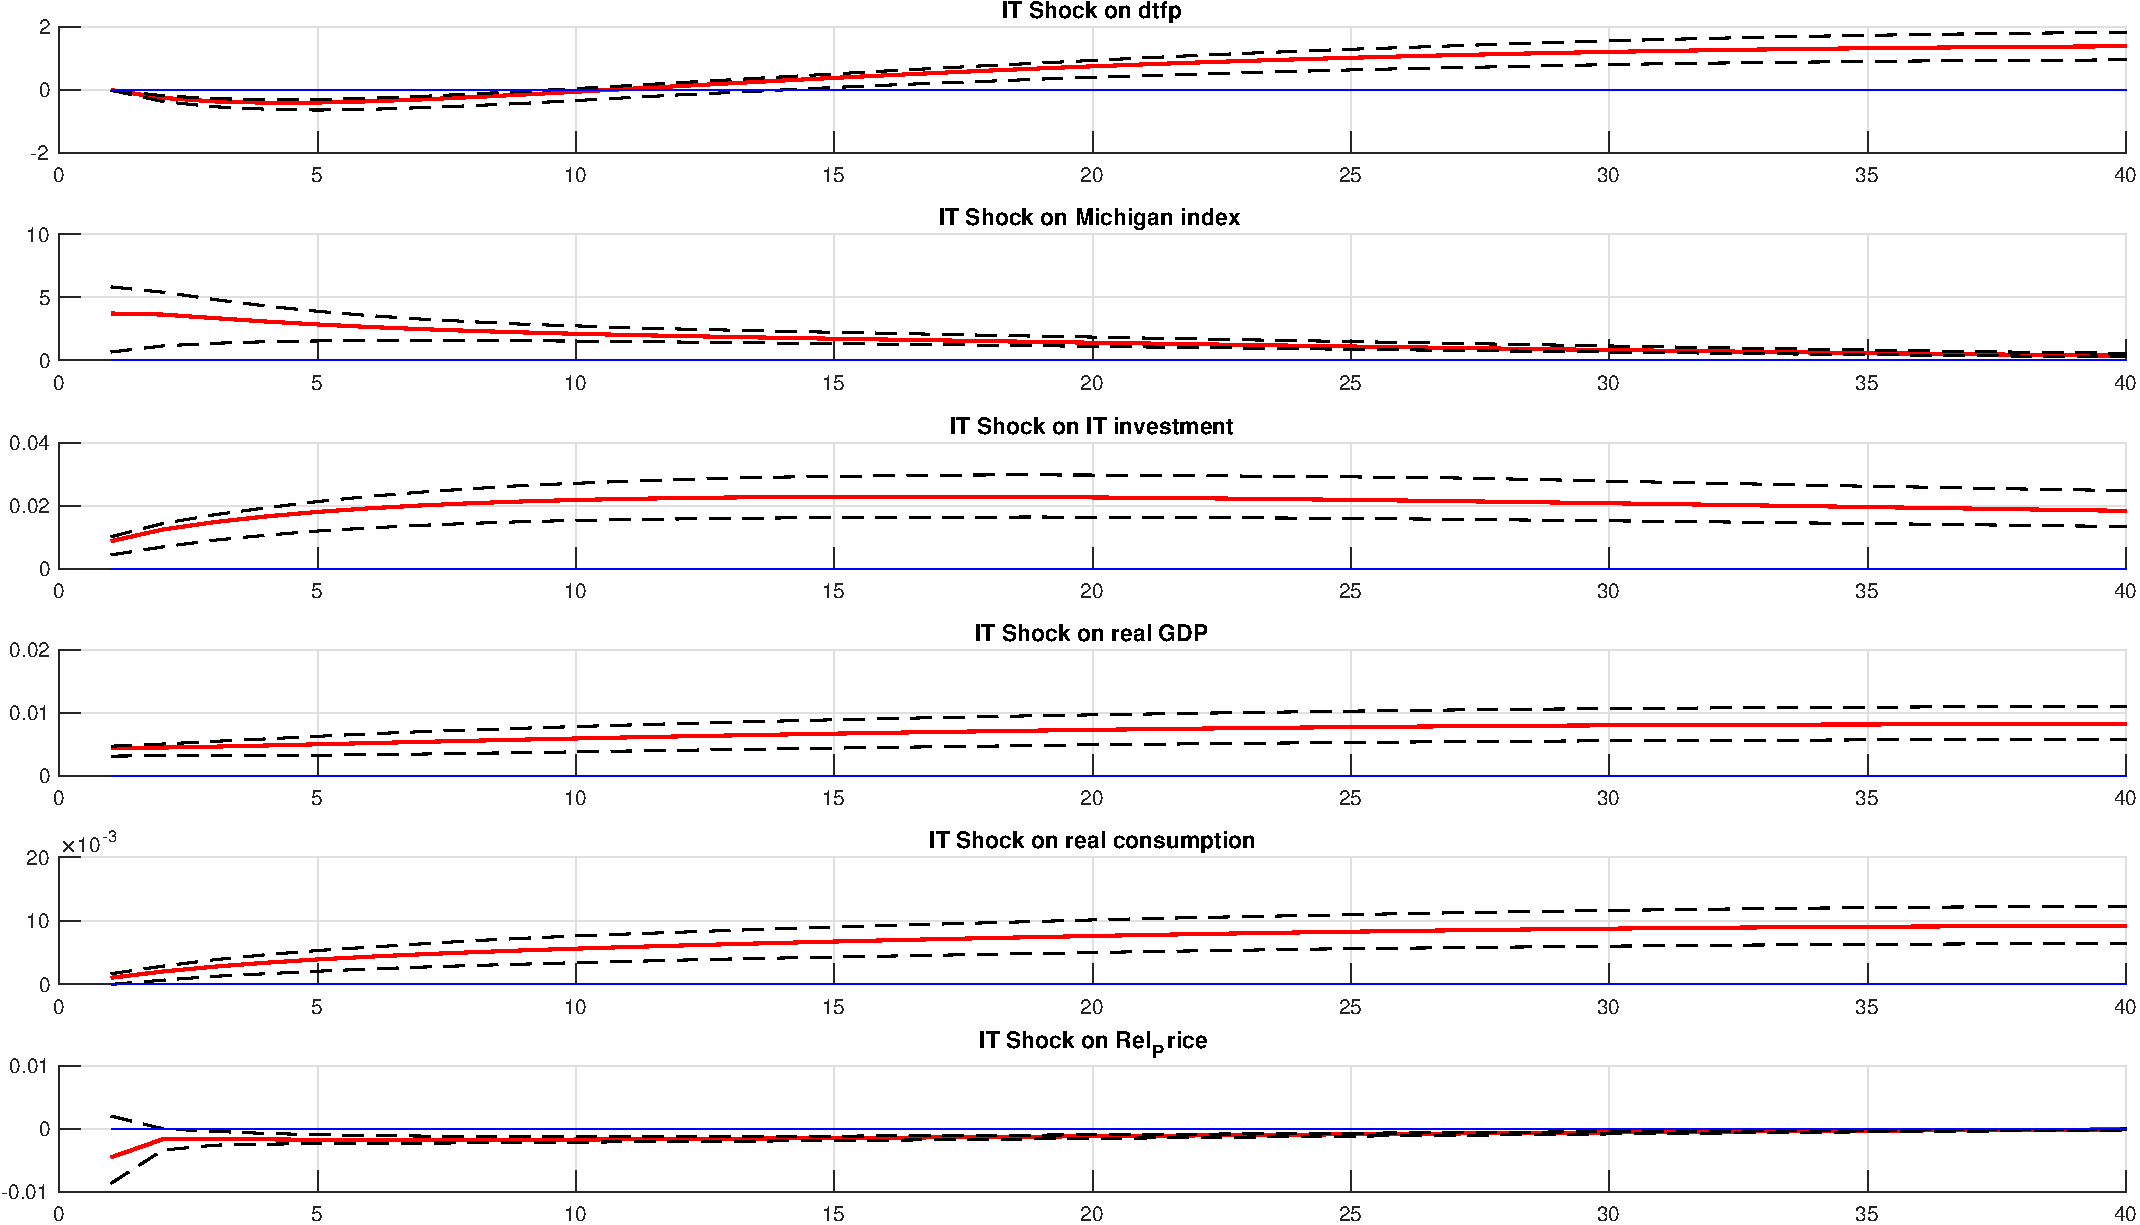
\includegraphics[width=8.5cm]{\ourFigPath Figures/fig_IT_Shock_Ryan_two_stepsID_24-Nov-2017_18_56_23}}
\end{figure}


%%%%%%%%
% LR hor of 80 - 
\newpage
\subsection{Relative prices LR horizon 80}
	\noindent Time it took, for 500 bootstrap, Mac: 81 min
	
	\
	
	\noindent  'News'       'IT'        'Total' 
	
         \noindent  '0.044546'    '0.69612'    '0.74067'
         
         \
         
         \begin{small}
	\begin{tabular}{lccc}
	\hline
		& News & IT & Total \\
		\hline
		Share of TFP FEV explained & 0.0 & 0.7 & 0.7 \\
		\hline
	\end{tabular}
\end{small}

         
         \

\begin{figure}[h!]
\centering
\subfigure[News]{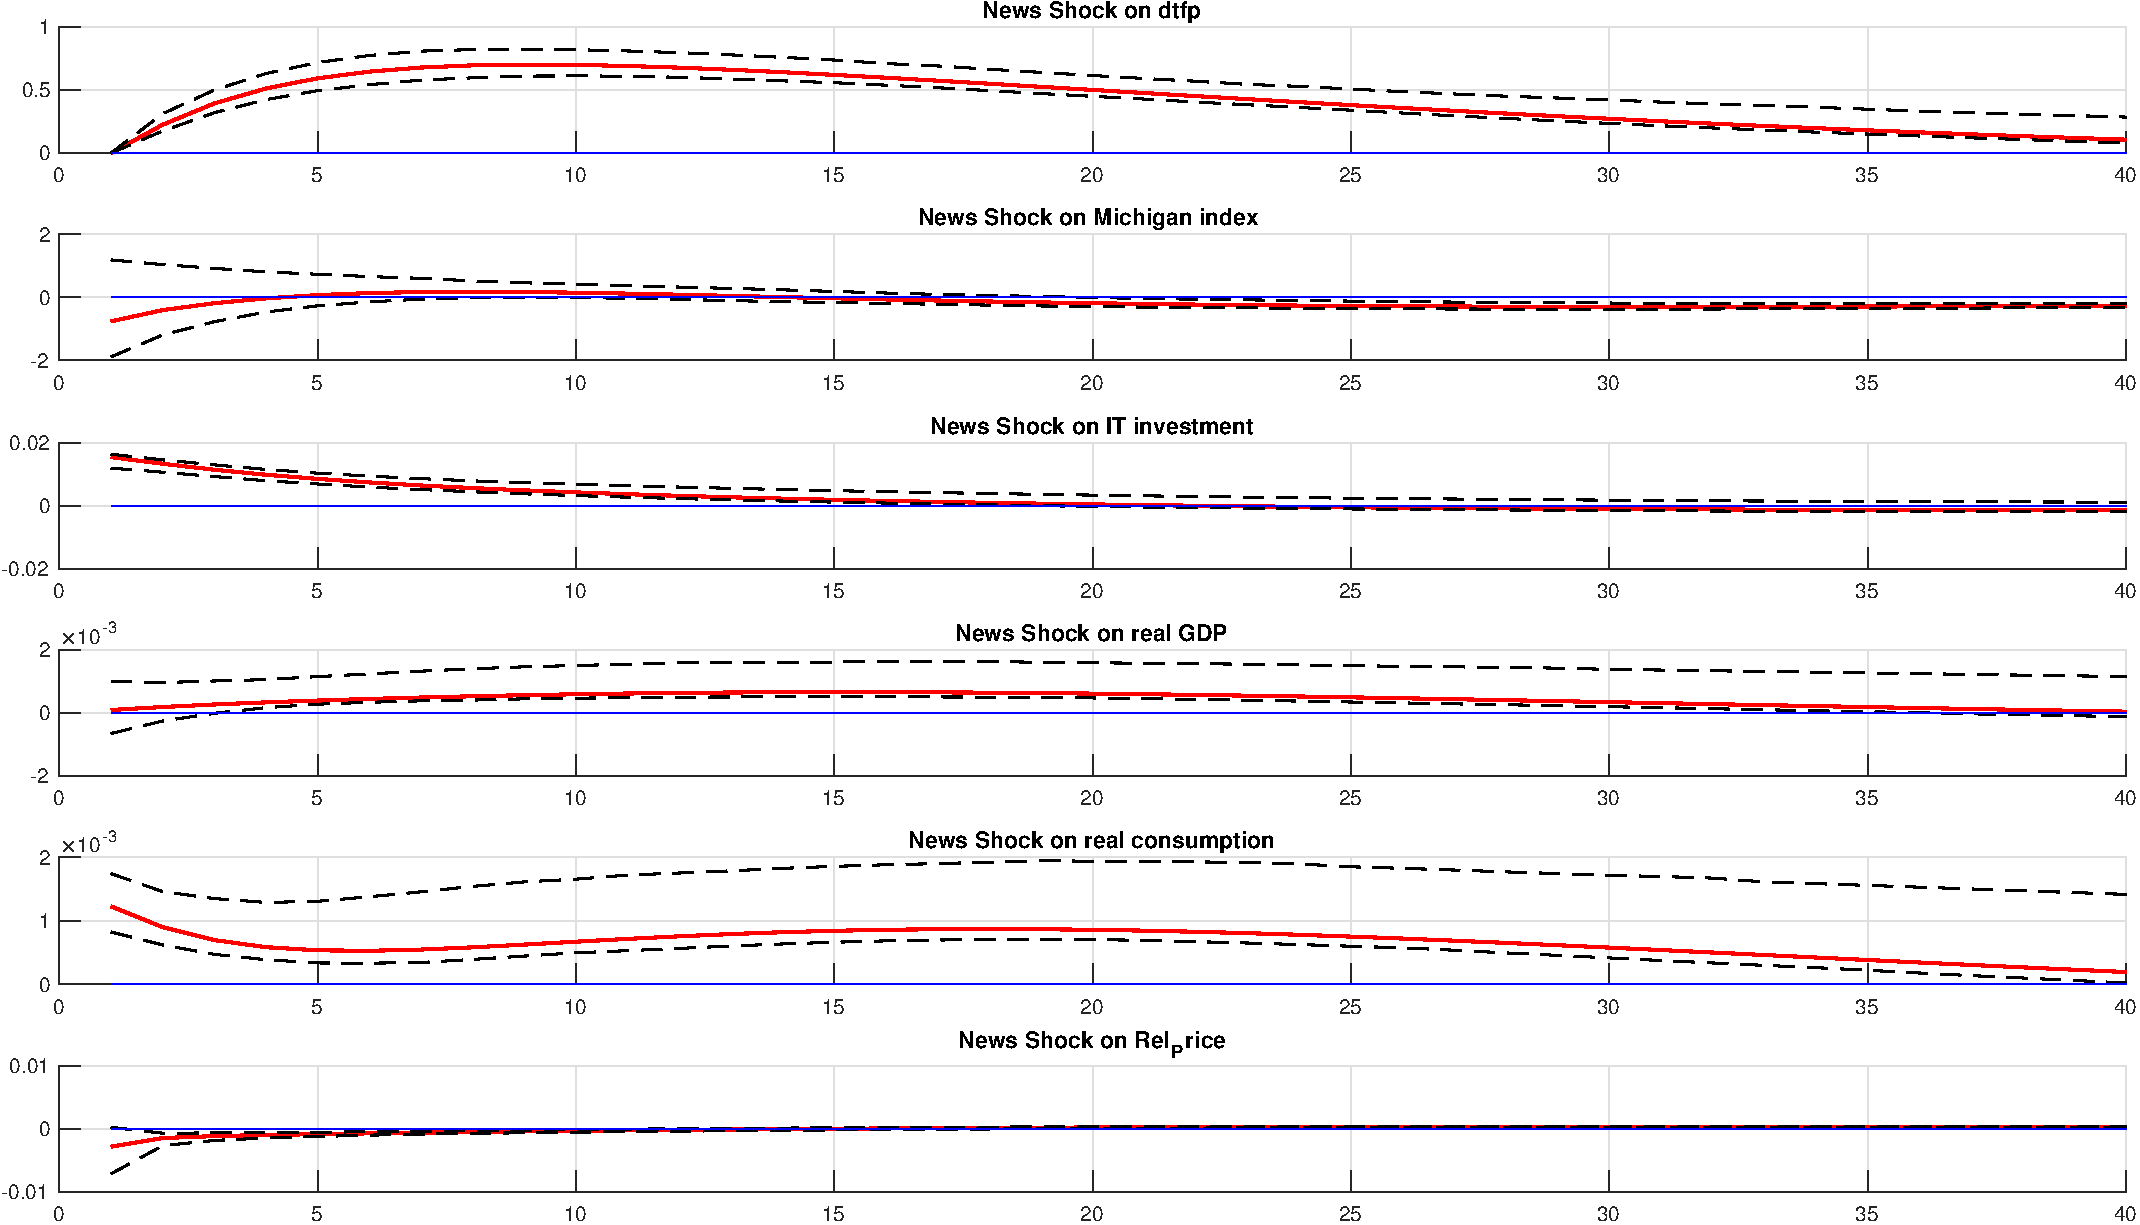
\includegraphics[width=8.5cm]{\ourFigPath Figures/fig_News_Shock_Ryan_two_stepsID_24-Nov-2017_21_59_10}} \hspace{.2in%
} 
\subfigure[IT]{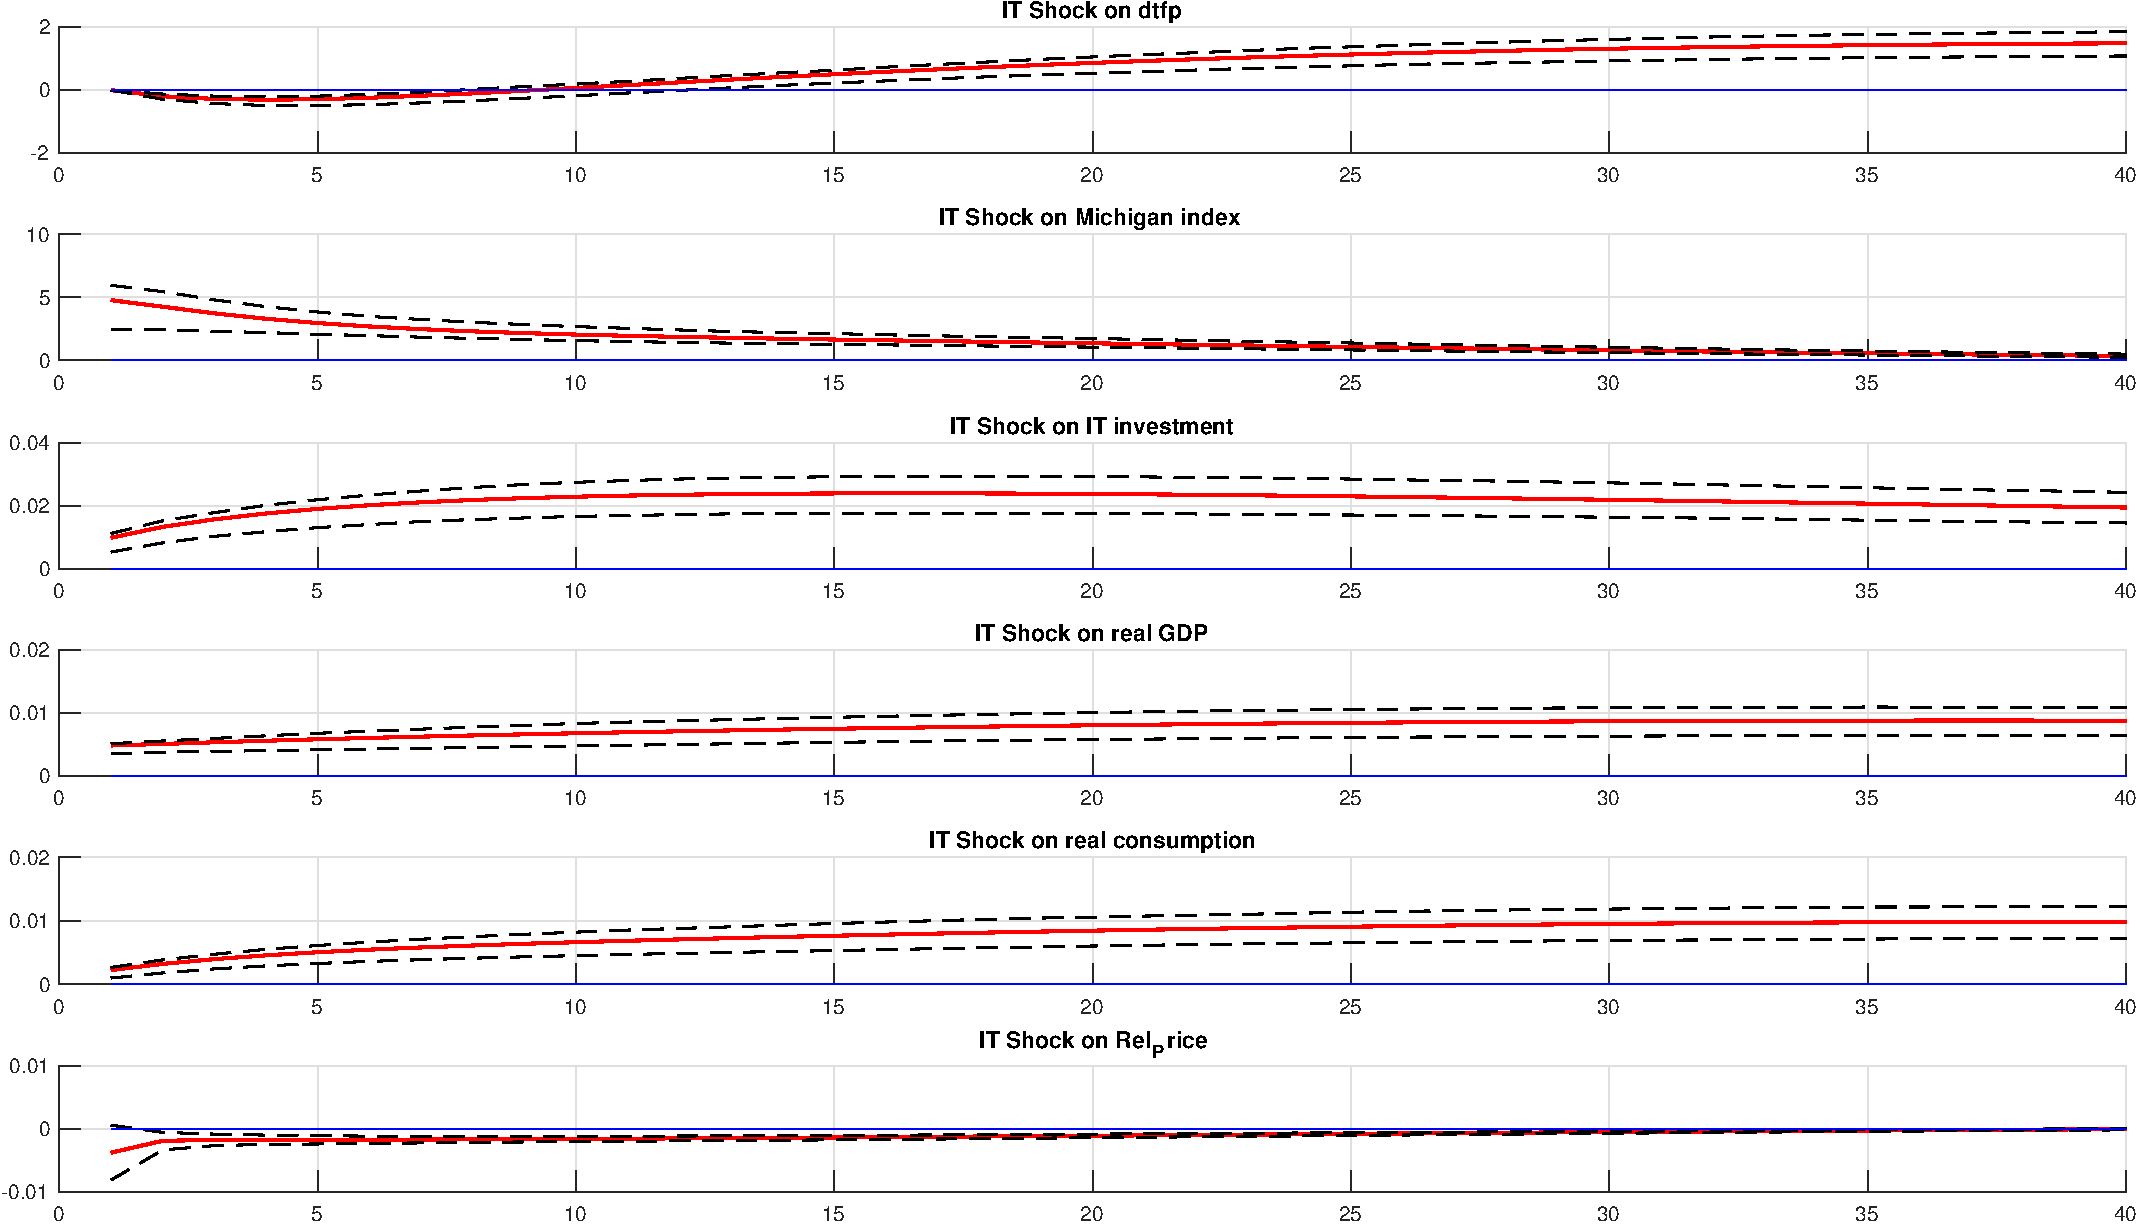
\includegraphics[width=8.5cm]{\ourFigPath Figures/fig_IT_Shock_Ryan_two_stepsID_24-Nov-2017_21_59_14}}
\end{figure}
 
%%%%%%%%
%two lags instead of one (back to LR hor = 8)

%%%%%%%%
% adding stock prices

%%%%%%%%
% removing consumption

%%%%%%%%
% and/or adding investment 
        
%%%%%%%%
% Capital prices
\newpage
	\subsection{Capital prices LR horizon 8}
	\noindent Time it took, for 500 bootstrap, Mac: 12 min
	
	\noindent  Time it took, for 500 bootstrap, server (w/o parpool): 30 min

	
	\noindent  'News'       'IT'        'Total' 
	
         \noindent  '0.40843'    '0.23982'    '0.64824'

	
	\begin{small}
	\begin{tabular}{lccc}
	\hline
		& News & IT & Total \\
		\hline
		Share of TFP FEV explained & 0.4 & 0.2 & 0.6 \\
		\hline
	\end{tabular}
\end{small}

	
	\begin{figure}[h!]
\centering
\subfigure[News]{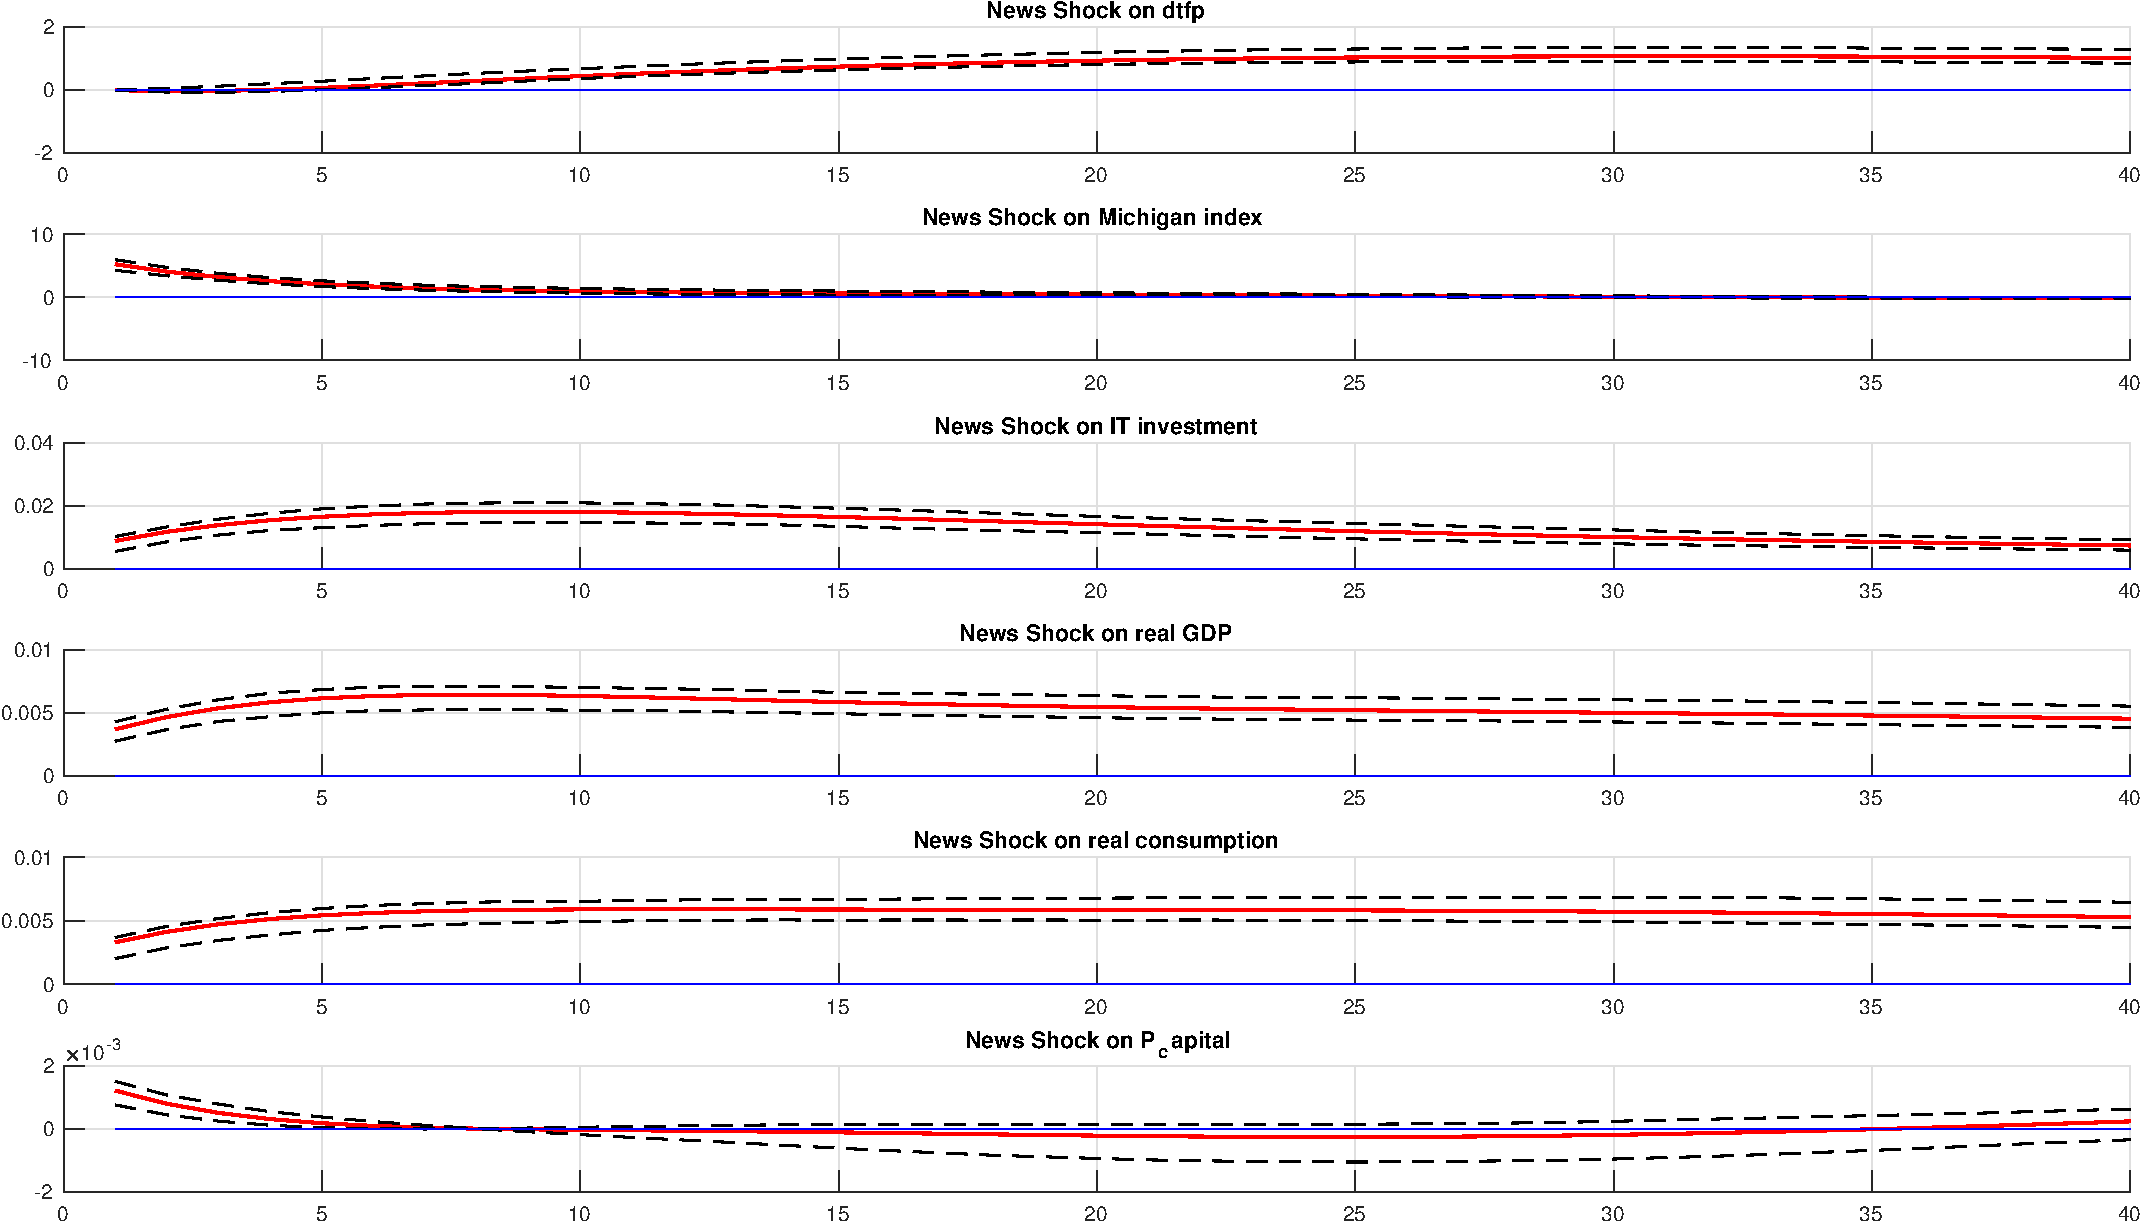
\includegraphics[width=8.5cm]{\ourFigPath Figures/fig_News_Shock_Ryan_two_stepsID_24-Nov-2017_16_17_15}} \hspace{.2in%
} 
\subfigure[IT]{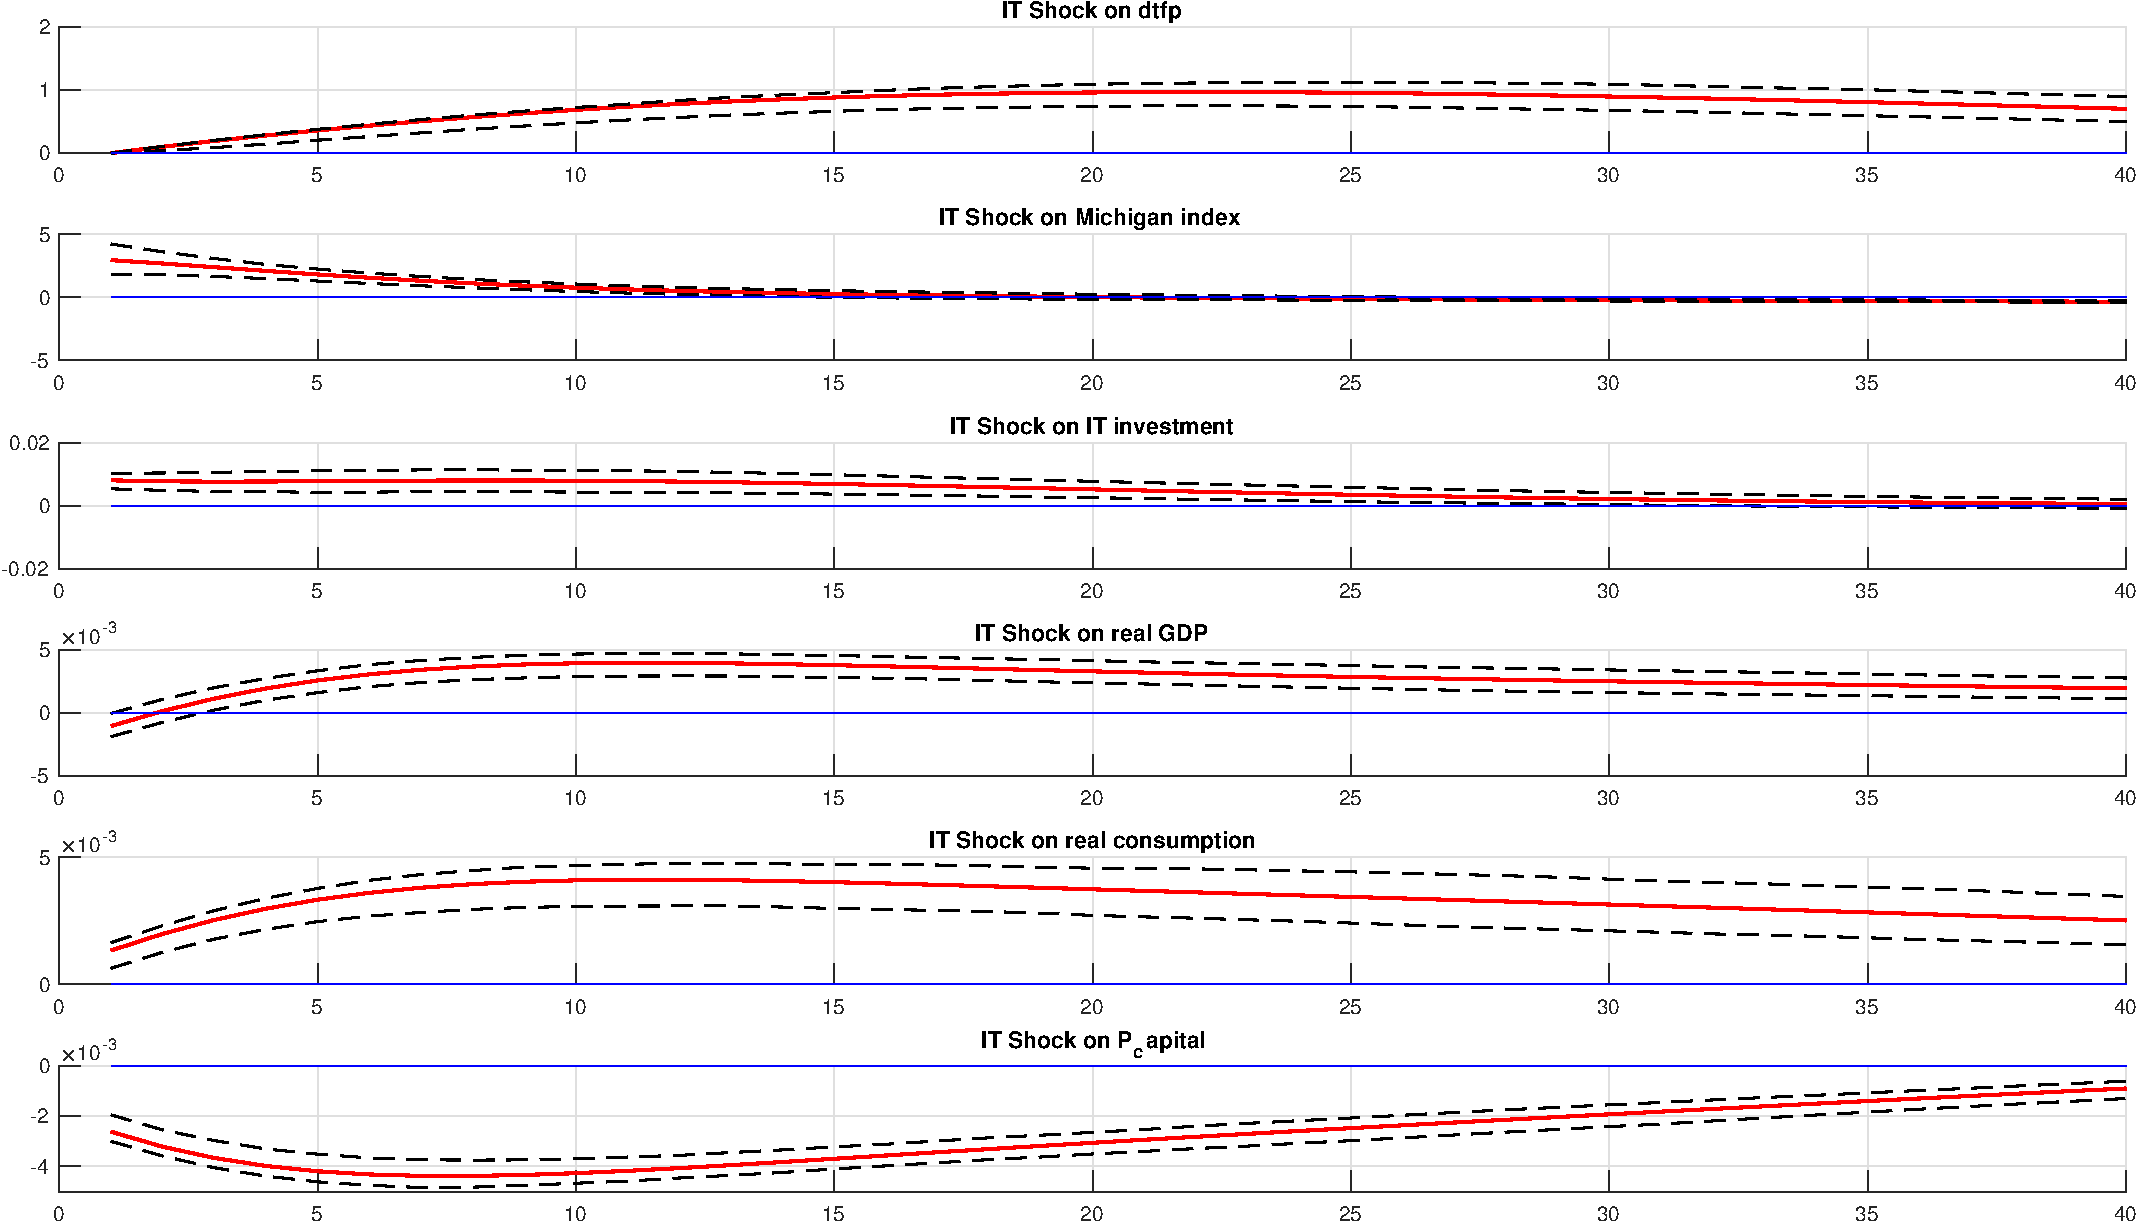
\includegraphics[width=8.5cm]{\ourFigPath Figures/fig_IT_Shock_Ryan_two_stepsID_24-Nov-2017_16_17_19}}
\end{figure}
	
	
		
	
	
\end{document}

